\RequirePackage{ifpdf}
	\ifpdf	
		\documentclass[pdftex]{article}
		%\usepackage[colorlinks, linkcolor=black, pdftex, plainpages=false, hyperindex, %pdfview=FitBH]{hyperref}
		\RequirePackage{color} 
	\else
		\documentclass[10pt]{article} 
		\usepackage{nohyperref}		
	\fi

\usepackage[utf8]{inputenc}
\usepackage[T1]{fontenc}
\usepackage[left=1.5cm, top=1.3cm, textwidth=18.6cm, textheight=27cm]{geometry}
\geometry{paper=a4paper}
\usepackage{graphicx}
\usepackage{titling}
\usepackage{abstract}
\usepackage{fancyhdr}
\usepackage{framed}

\lhead{} \chead{} \rhead{}
\lfoot{\emph{Research Skills and Methodology, 2014/2015}} \cfoot{} \rfoot{\thepage}
\renewcommand{\headrulewidth}{0pt}
\renewcommand{\footrulewidth}{0.4pt}
\pagestyle{fancy}

\posttitle{\par\end{center}}
\preauthor{\begin{center} \large \begin{tabular}[t]{c}}
\postauthor{\end{tabular}\par\end{center}}
\predate{} \postdate{}
\date{}

\pretitle{
\includegraphics[width=.55\textwidth]{eka-pl.png}\par\vspace{1ex}\begin{center}\huge}

\newcommand{\eng}[1]{(ang.\ \emph{#1})}

\title{Metaheuristic Chess Artificial Intelligence}
\author{Maciej Borkowski\\ 195968@student.pwr.edu.pl \and Paweł Pałus\\ zzzzzz@student.pwr.edu.pl  \and Mariusz Waszczyński\\  xxxxxx@student.pwr.edu.pl }

\begin{document}
\thispagestyle{empty}
\twocolumn[
	\maketitle
	\begin{abstract}
something something something something something something something something something something something something something something something something something something something 
	{
		\begin{description} 
		\item[Index Terms:] \emph{chess, metaheuristics, artificial intelligence, ant colony, genetic, simulated annealing}
		\end{description}
	}
	\end{abstract}
	\vspace{2em}
]

\section{Introduction}
\label{sec:introduction}

Hello

\section{Optimization Problem}
\label{sec:problem}

The problem describes a standard game of chess, with a square board of 64 fields. Two players have to consecutively move a piece the board onto another field according to complex, well-defined rules. Our task is to find the series of movements in a game of chess that gives the best chance of winning the game in the end. The starting position of pieces can be arbitrary.

\subsection{Mathematical model}
\label{sec:model}

From card, expand on it

\section{Experimentation system}
\label{sec:project}

About the application

\subsection{UCI}
\label{sec:uci}

\subsubsection{Firenzina}
\label{sec:firenzina}

\subsection{GUI}
\label{sec:uci}

About the GUI

\section{Algorithms}
\label{sec:project}

\subsection{Ant colony (Maciej Borkowski)}
\label{sec:ant}

\subsubsection{Idea}
For ant colony search algorithm a mapping is created between a placement of chess pieces on a chessboard and a list of possible moves the current player is able to do, when provided such board. Each move on this list is additionally annotated with a real value, which describes the fitness of the move. Moves with higher fitness ought to yield us better results. Such mapping is called a pheromone and a set of them pheromones (Figure \ref{fig:pheromones}).

\begin{figure*}[!htb]
	\centering
	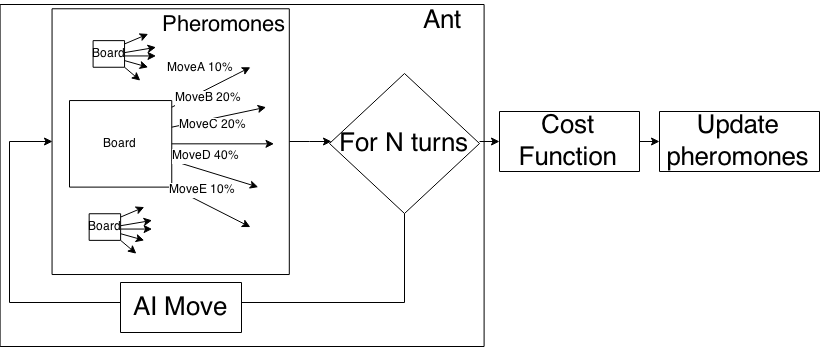
\includegraphics[width=1\textwidth]{ant/pheromones.png} 
	\caption{Diagram of the implemented ant colony search algorithm with visualisation of pheromones for one iteration with one ant}
	\label{fig:pheromones}
\end{figure*}

Ant is defined here as a chess player, that uses pheromones to choose a move when it is metaheuristic's time to make a choice of movement. Ant can be a part of a colony, in which case the colony provides the pheromones or it can be independent (used for Greedy Mode). Pheromones can be saved to and loaded from a file. When an ant finds itself on a board that has not yet been added to pheromones a new pheromone is created (possible moves for the board are computed and assigned equal real values).

 Ant can work in one of two modes: 
\begin{itemize}
 	\item Adventurous Mode \hfill \\
		Used for learning. In this case the ant works for the betterment of its colony. It chooses moves randomly, according to the values of pheromones. This strategy improves the pheromones, by visiting a wide range of possible boards, which results in frequent updates and addition of new pheromones. The probability of choosing move M (with real value v):
\begin{equation}
\label{eq:choosingequation}
	P(M) = \frac{v_m + |min(V)|}{\sum V + n|(min(V))|}
\end{equation}
where~$V$ are all values in a given pheromone,~$v_m$ the value for move and~$n$ is the length of~$V$.

	\item Greedy Mode \hfill \\
		Used for testing and real games. In this case the ant plays for the best end result in its game. Ant chooses a move from the pheromone with the highest value to choose the best move in each turn.
\end{itemize}

The process of learning consists of many iterations of ants in Adventurous Mode working as a colony. Each iteration amounts to a few phases:
\begin{enumerate}
 	\item Start new games and wait for them to end \hfill \\
		Each ant plays one game of chess and remembers all boards it has run across, all moves it has chosen to do and the
the cost function of the series of movements (value of cost function for last board).
	\item Update pheromones \hfill \\
		For each ant the pheromones connected to visited boards are updated by a fraction of the value of cost function of the whole series of movements.
\begin{equation}
	v_{new} = v_{old} + \frac{i}{m} cost
\end{equation}
where~$v_{new}$ is the new value, ~$v_{old}$ is the old value,~$i$ is the index of the movement in this series of movements, ~$m$ is the length of the series of movements and~$cost$ ist the value of cost function.
	\item Dissipate pheromones \hfill \\
		Pheromone for each of the boards that has been visited at least once by any ant in this game is decreased by multiplying the value by a parameter.
\begin{equation}
\label{eq:dissipationequation}
	v_{new} =  v_{old} *  (1 - dissipation)
\end{equation}
where~$v_{new}$ is the new value, ~$v_{old}$ is the old value and~$dissipation$ is a parameter. 

\end{enumerate}

Pheromones can be saved to a file. The file consists of a list of pheromones, each is described with two lines:
\begin{enumerate}
 	\item String representation of a board, left to right, bottom to up, where \# means no chessman, upper case letters mean white chessmen and lower case letters mean black chessmen \hfill \\
	\item A list of moves. Each move is described by five integer values. First two are the coordinates of chessman to move, third and fourth where to move the chessman to, the fifth is a special value used for promotion (when a pawn becomes another chess piece) and the sixth a real value of pheromone describing its effectiveness. \hfill \\
\end{enumerate}

\subsubsection{Experiments}

Firstly, it has to be accentuated that chess is a complex game, the number of possible boards that have to be remembered in pheromones is huge and for each ant move another move has to be done by external Artificial Intelligence. Because of these reasons the learning phase of this metaheuristic takes a very long time. To get results appearing significantly different from completely random ones, hours have to be spent on learning. This makes it very difficult and time-consuming to experiment with parameters properly.

\begin{figure}[!htb]
	\centering
	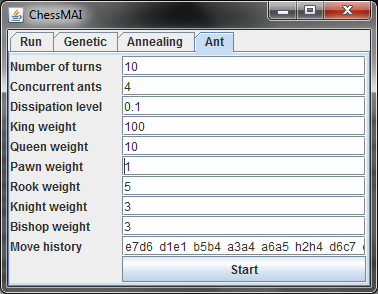
\includegraphics[width=0.5\textwidth]{ant/antapplication.png} 
	\caption{Ant colony dialog boxes}
	\label{fig:antapplication}
\end{figure}

For the experiments the parametrization of many ant search specific variables has been put into dialog boxes in the application(Figure \ref{fig:antapplication}). This way user can change these values easily and create his own colonies. The user-available parameters are as follows:

\begin{itemize}
 	\item Number of turns \hfill \\
The number of turns for each iteration. Each iteration consists of an all concurrent ants playing one game of chance up to a win, lose, draw or the artificial end of game, when it takes too long. This parameter should be kept low if we want the learning phase to take less time and if we want ants to have more broad "knowledge" of possible moves in the beggining of the game. 
	\item Concurrent ants \hfill \\
The number of ants playing a game in each iteration. The more of them the longer each iteration takes.
 	\item Dissipation level \hfill \\
The dissipation parameter of ant search algorithm dissipation equation (Equation~\ref{eq:dissipationequation}).
	\item Piece weight \hfill \\
Each piece has its own weight used in cost function (Equation~\ref{eq:costfunction})
	\item Move history \hfill \\
This parameter sets the starting position of the game from any point, provided a valid chess move history. Each ant in each iteration starts its game from this point and plays up until the end of the game (including the end of maximum number of turns defined as another parameter)
\end{itemize}

The more obvious rules had to be applied to get to the point of metaheuristic being better than a random algorithm and able to win one game out of hundreds when playing against the artificial intelligence. Most importantly the weight of king should far bigger than other figures, the number of turns small, and a move history provided that gives a possibility of winning in a few turns. Increasing the number of concurrent ants and, at the same time, the dissipation level makes the results possibly even better but by a very small margin at the cost of a longer learning phase (making it difficult to test).


\subsubsection{Result}

Meddling in all of these parameters proved to be insufficient in obtaining better results. After careful debugging of the application, the conclusion has been made, that the possible reason for improvement could be to increase the probability of choosing good moves instead of dwell on the bad moves. Even though the move choosing equation (Equation~\ref{eq:choosingequation}) gives more probability to good moves, it is not very significant to the sum of all the probabilities, because there are generally a lot of bad moves. One of the ideas was to sum up the logarithms of values in equation, which is often a way of dealing with those kind of issues. This however only made the values of pheromones more close to each other so the probability of choosing a good move didn't really change that much. 

The really important change was observed when the Equation~\ref{eq:choosingequation} was modified to one with a "tolerance" factor multiplied by each value except the best one. This way the probability of choosing the best move in training is big, enabling  the colony to thoroughly establish how good of a situation on the board it results in. This can quite easily culminate in a fall into a local maximum of cost function, but it is not a bad situation to be in chess - at least we end up in a better situation than before. Additionally to really fall into a local maximum the moves have to contain a lot of weight gain, so it would be most probably a checkmate anyway, which is, for all intents and purposes, a global maximum. Indeed, if a winning sequence of moves has been established in this version the colony started winning very often.

\subsection{Genetic algorithm}
\label{sec:genetic}

\subsubsection{what?}
\subsubsection{gui/experiment}
\subsubsection{result}

\subsection{Simulated Annealing}
\label{sec:annealing}

\subsubsection{what?}
\subsubsection{gui/experiment}
\subsubsection{result}

\section{Improvements}
\label{sec:improvements}

 - put all the variables/modes etc in GUI
 - adding new engines and randomize their use between moves


\section{Conclusion}
\label{sec:conclusion}


It was fun / not fun.

\begin{thebibliography}{99}

\bibitem{comparison} \textsc{Vecek, N. ; Crepinsek, M. ; Mernik, M. ; Hrncic, D.}, A comparison between different chess rating systems for ranking evolutionary algorithms 
\bibitem{ant} \textsc{Dorigo, M. ; Maniezzo, V. ; Colorni, A.}, Ant system: optimization by a colony of cooperating agents 
\bibitem{genetic} \textsc{David, O.E. ; van den Herik, H.J. ; Koppel, M. ; Netanyahu, N.S. }, Genetic Algorithms for Evolving Computer Chess Programs 
\bibitem{annealing} \textsc{S. Kirkpatrick; C. D. Gelatt; M. P. Vecchi.}, Optimization by Simulated Annealing 
\bibitem{uci} \textsc{R. Huber, S. Meyer-Kahlen}, Universal Chess Interface, http://www.shredderchess.com/chess-info/features/uci-universal-chess-interface.html, 2015/06/01

\end{thebibliography}
\end{document}
